\documentclass[twoside, a4paper,12pt, tikz]{scrartcl}
\usepackage{pdflscape}
\usepackage{tabularx}
\usepackage{lipsum}
\usepackage{color}
\usepackage{enumitem,amssymb, amsmath}
\usepackage{xcolor}
\usepackage{tikz}
\usepackage{tkz-euclide}
\usepackage{float}
\usepackage{fancyhdr}
\usepackage{titlesec}  
\pagestyle{fancy}% Opcional: mejor control sobre títulos

% Activar encabezados personalizados
\pagestyle{fancy}
\fancyhf{} % Limpiar encabezados y pies

% Texto fijo + nombre de sección en el encabezado interior
\fancyhead[LE]{Agenda — \nouppercase{\leftmark}} % L = lado izquierdo, E = página par
\fancyhead[RO]{Agenda — \nouppercase{\leftmark}} % R = lado derecho, O = página impar

% Número de página en el borde exterior
\fancyfoot[LE,RO]{\thepage}

% Actualizar \leftmark con el nombre de la sección
\renewcommand{\sectionmark}[1]{\markboth{#1}{}}

% Opcional: hacer que las secciones no estén en mayúsculas automáticamente
\usepackage{sectsty}
\allsectionsfont{\normalfont}


\newcommand\Vtextvisiblespace[1][.3em]{%
  \mbox{\kern.06em\vrule height.3ex}%
  \vbox{\hrule width#1}%
  \hbox{\vrule height.3ex}}
\newcommand{\checkbox}{ {\fboxsep=-.2pt\fbox{\rule{0pt}{2ex}\rule{2ex}{0pt}}}}

\newcommand{\subtablaDescrip}{ \begin{tabular}{ll}&\\ prioridad: & \Vtextvisiblespace[2em] \\ dificultad: & \Vtextvisiblespace[2em]\\&\\ \end{tabular}}

\definecolor{calendarHeader}{RGB}{232,238,245}
\definecolor{calendarWeekend}{RGB}{244,239,229}
\definecolor{calendarBorder}{RGB}{110,122,135}

\newcommand{\calendarMeta}[2]{%
  {\footnotesize #1\par #2\par}%
}

\newcommand{\calendarMoonCorner}[1]{%
  \hfill #1%
}

\newcommand{\calendarDayBlock}[5]{%
\fcolorbox{calendarBorder}{white}{%
\begin{minipage}[t][0.44\textheight][t]{\dimexpr\linewidth-2\fboxsep-2\fboxrule\relax}
\colorbox{calendarHeader}{\parbox{\dimexpr\linewidth-2\fboxsep\relax}{\strut\textbf{\sffamily #1}\hfill #2}}%
\vspace{0.8ex}
\calendarMeta{#3}{#4}
\vfill
\calendarMoonCorner{#5}
\end{minipage}}%
}

\newcommand{\calendarWeekendBlock}[8]{%
\fcolorbox{calendarBorder}{white}{%
\begin{minipage}[t][0.44\textheight][t]{\dimexpr\linewidth-2\fboxsep-2\fboxrule\relax}
\colorbox{calendarWeekend}{\parbox{\dimexpr\linewidth-2\fboxsep\relax}{\strut\textbf{\sffamily Sábado}\hfill #1}}%
\vspace{0.6ex}
\calendarMeta{#2}{#3}
\vfill
\calendarMoonCorner{#4}
\vspace{0.6ex}
\hrule
\vspace{0.6ex}
\colorbox{calendarWeekend}{\parbox{\dimexpr\linewidth-2\fboxsep\relax}{\strut\textbf{\sffamily Domingo}\hfill #5}}%
\vspace{0.6ex}
\calendarMeta{#6}{#7}
\vfill
\calendarMoonCorner{#8}
\end{minipage}}%
}

\begin{document}
 
\section*{Periodo Aug 24, 2026, 4 semanas }

\newpage

\section*{Gráfica}

\begin{figure}[H]
\centering
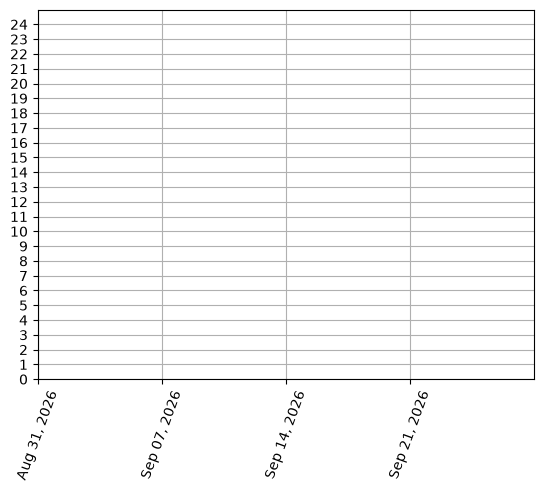
\includegraphics[scale=1]{graph.png}
\end{figure}

  \newpage
  $\;$
  \newpage
\section*{Semana Aug 24, 2026 -- Aug 30, 2026}
\markboth{Semana Aug 24, 2026 -- Aug 30, 2026}{}
\thispagestyle{empty}
\noindent
\begin{tabularx}{\linewidth}{|X|c c|}
    \hline
  \textbf{Tarea} & \textbf{descripción} & \textbf{proceso}\\
  \hline
   1.\vspace{4ex} &      \subtablaDescrip     & $\square\square\square\square\square$ \\
  \hline
  2.\vspace{4ex} &      \subtablaDescrip     & $\square\square\square\square\square$ \\
  \hline
  3.\vspace{4ex} &      \subtablaDescrip     & $\square\square\square\square\square$ \\
  \hline
  4.\vspace{4ex} &      \subtablaDescrip     & $\square\square\square\square\square$ \\
  \hline
  5.\vspace{4ex} &      \subtablaDescrip     & $\square\square\square\square\square$ \\
  \hline
  6.\vspace{4ex} &      \subtablaDescrip     & $\square\square\square\square\square$ \\
  \hline
  7.\vspace{4ex} &      \subtablaDescrip     & $\square\square\square\square\square$ \\
  \hline
  8.\vspace{4ex} &      \subtablaDescrip     & $\square\square\square\square\square$ \\
  \hline
  9.\vspace{4ex} &      \subtablaDescrip     & $\square\square\square\square\square$ \\
  \hline
  10.\vspace{4ex} &      \subtablaDescrip     & $\square\square\square\square\square$ \\
  \hline
\end{tabularx}

\newpage



\begin{center}
\begin{tabular}{ll}
\textbf{Facilidades / dificultades} & \textbf{Objetivos} \\
\fcolorbox{black!50!black}{white}{
\begin{tabular}{c}
  \phantom{Lorem ipsum dolor sit amet, consectetur}\\
  \phantom{Lorem ipsum dolor sit amet, consectetur}\\
  \phantom{Lorem ipsum dolor sit amet, consectetur}\\
  \phantom{Lorem ipsum dolor sit amet, consectetur}\\
  \phantom{Lorem ipsum dolor sit amet, consectetur}\\
  \phantom{Lorem ipsum dolor sit amet, consectetur}\\
  \phantom{Lorem ipsum dolor sit amet, consectetur}\\
  \phantom{Lorem ipsum dolor sit amet, consectetur}\\
\end{tabular}

} &
\fcolorbox{black!50!black}{white}{
\begin{tabular}{c}
  \phantom{Lorem ipsum dolor sit amet, consectetur}\\
  \phantom{Lorem ipsum dolor sit amet, consectetur}\\
  \phantom{Lorem ipsum dolor sit amet, consectetur}\\
  \phantom{Lorem ipsum dolor sit amet, consectetur}\\
  \phantom{Lorem ipsum dolor sit amet, consectetur}\\
  \phantom{Lorem ipsum dolor sit amet, consectetur}\\
  \phantom{Lorem ipsum dolor sit amet, consectetur}\\
  \phantom{Lorem ipsum dolor sit amet, consectetur}\\
\end{tabular}
} \\
\end{tabular}
\end{center}

\begin{center}
\textbf{Reflexiones}\\ \vspace{3ex}
\fcolorbox{black!50!black}{white}{
\begin{tabular}{l}
\phantom{Lorem ipsum dolor sit amet, consectetur Lorem  Lorem ipsum dolor sit amet, consectetur}\\
\phantom{Lorem ipsum dolor sit amet, consectetur}\\
\phantom{Lorem ipsum dolor sit amet, consectetur}\\
\phantom{Lorem ipsum dolor sit amet, consectetur}\\
\phantom{Lorem ipsum dolor sit amet, consectetur}\\
\phantom{Lorem ipsum dolor sit amet, consectetur}\\
\phantom{Lorem ipsum dolor sit amet, consectetur}\\
\phantom{Lorem ipsum dolor sit amet, consectetur}\\
\phantom{Lorem ipsum dolor sit amet, consectetur}\\
\phantom{Lorem ipsum dolor sit amet, consectetur}\\
\phantom{Lorem ipsum dolor sit amet, consectetur}\\
\end{tabular}
}
\end{center}
\vspace{5ex}

\begin{center}
\textbf{Notas}\\ \vspace{3ex}
\fcolorbox{black!50!black}{white}{
    \begin{tabular}{l}
    \phantom{Lorem ipsum dolor sit amet, consectetur Lorem  Lorem ipsum dolor sit amet, consectetur}\\
    \phantom{Lorem ipsum dolor sit amet, consectetur}\\
    \phantom{Lorem ipsum dolor sit amet, consectetur}\\
    \phantom{Lorem ipsum dolor sit amet, consectetur}\\
    \phantom{Lorem ipsum dolor sit amet, consectetur}\\
    \phantom{Lorem ipsum dolor sit amet, consectetur}\\
    \phantom{Lorem ipsum dolor sit amet, consectetur}\\
    \phantom{Lorem ipsum dolor sit amet, consectetur}\\
    \phantom{Lorem ipsum dolor sit amet, consectetur}\\
    \phantom{Lorem ipsum dolor sit amet, consectetur}\\
    \phantom{Lorem ipsum dolor sit amet, consectetur}\\
    \end{tabular}
  }
\end{center}

\vspace{5ex}
Resultado semana: \Vtextvisiblespace[2em]

\newpage
\section*{Semana Aug 31, 2026 -- Sep 06, 2026}
\markboth{Semana Aug 31, 2026 -- Sep 06, 2026}{}
\thispagestyle{empty}
\noindent
\begin{tabularx}{\linewidth}{|X|c c|}
    \hline
  \textbf{Tarea} & \textbf{descripción} & \textbf{proceso}\\
  \hline
   1.\vspace{4ex} &      \subtablaDescrip     & $\square\square\square\square\square$ \\
  \hline
  2.\vspace{4ex} &      \subtablaDescrip     & $\square\square\square\square\square$ \\
  \hline
  3.\vspace{4ex} &      \subtablaDescrip     & $\square\square\square\square\square$ \\
  \hline
  4.\vspace{4ex} &      \subtablaDescrip     & $\square\square\square\square\square$ \\
  \hline
  5.\vspace{4ex} &      \subtablaDescrip     & $\square\square\square\square\square$ \\
  \hline
  6.\vspace{4ex} &      \subtablaDescrip     & $\square\square\square\square\square$ \\
  \hline
  7.\vspace{4ex} &      \subtablaDescrip     & $\square\square\square\square\square$ \\
  \hline
  8.\vspace{4ex} &      \subtablaDescrip     & $\square\square\square\square\square$ \\
  \hline
  9.\vspace{4ex} &      \subtablaDescrip     & $\square\square\square\square\square$ \\
  \hline
  10.\vspace{4ex} &      \subtablaDescrip     & $\square\square\square\square\square$ \\
  \hline
\end{tabularx}

\newpage



\begin{center}
\begin{tabular}{ll}
\textbf{Facilidades / dificultades} & \textbf{Objetivos} \\
\fcolorbox{black!50!black}{white}{
\begin{tabular}{c}
  \phantom{Lorem ipsum dolor sit amet, consectetur}\\
  \phantom{Lorem ipsum dolor sit amet, consectetur}\\
  \phantom{Lorem ipsum dolor sit amet, consectetur}\\
  \phantom{Lorem ipsum dolor sit amet, consectetur}\\
  \phantom{Lorem ipsum dolor sit amet, consectetur}\\
  \phantom{Lorem ipsum dolor sit amet, consectetur}\\
  \phantom{Lorem ipsum dolor sit amet, consectetur}\\
  \phantom{Lorem ipsum dolor sit amet, consectetur}\\
\end{tabular}

} &
\fcolorbox{black!50!black}{white}{
\begin{tabular}{c}
  \phantom{Lorem ipsum dolor sit amet, consectetur}\\
  \phantom{Lorem ipsum dolor sit amet, consectetur}\\
  \phantom{Lorem ipsum dolor sit amet, consectetur}\\
  \phantom{Lorem ipsum dolor sit amet, consectetur}\\
  \phantom{Lorem ipsum dolor sit amet, consectetur}\\
  \phantom{Lorem ipsum dolor sit amet, consectetur}\\
  \phantom{Lorem ipsum dolor sit amet, consectetur}\\
  \phantom{Lorem ipsum dolor sit amet, consectetur}\\
\end{tabular}
} \\
\end{tabular}
\end{center}

\begin{center}
\textbf{Reflexiones}\\ \vspace{3ex}
\fcolorbox{black!50!black}{white}{
\begin{tabular}{l}
\phantom{Lorem ipsum dolor sit amet, consectetur Lorem  Lorem ipsum dolor sit amet, consectetur}\\
\phantom{Lorem ipsum dolor sit amet, consectetur}\\
\phantom{Lorem ipsum dolor sit amet, consectetur}\\
\phantom{Lorem ipsum dolor sit amet, consectetur}\\
\phantom{Lorem ipsum dolor sit amet, consectetur}\\
\phantom{Lorem ipsum dolor sit amet, consectetur}\\
\phantom{Lorem ipsum dolor sit amet, consectetur}\\
\phantom{Lorem ipsum dolor sit amet, consectetur}\\
\phantom{Lorem ipsum dolor sit amet, consectetur}\\
\phantom{Lorem ipsum dolor sit amet, consectetur}\\
\phantom{Lorem ipsum dolor sit amet, consectetur}\\
\end{tabular}
}
\end{center}
\vspace{5ex}

\begin{center}
\textbf{Notas}\\ \vspace{3ex}
\fcolorbox{black!50!black}{white}{
    \begin{tabular}{l}
    \phantom{Lorem ipsum dolor sit amet, consectetur Lorem  Lorem ipsum dolor sit amet, consectetur}\\
    \phantom{Lorem ipsum dolor sit amet, consectetur}\\
    \phantom{Lorem ipsum dolor sit amet, consectetur}\\
    \phantom{Lorem ipsum dolor sit amet, consectetur}\\
    \phantom{Lorem ipsum dolor sit amet, consectetur}\\
    \phantom{Lorem ipsum dolor sit amet, consectetur}\\
    \phantom{Lorem ipsum dolor sit amet, consectetur}\\
    \phantom{Lorem ipsum dolor sit amet, consectetur}\\
    \phantom{Lorem ipsum dolor sit amet, consectetur}\\
    \phantom{Lorem ipsum dolor sit amet, consectetur}\\
    \phantom{Lorem ipsum dolor sit amet, consectetur}\\
    \end{tabular}
  }
\end{center}

\vspace{5ex}
Resultado semana: \Vtextvisiblespace[2em]

\newpage
\section*{Semana Sep 07, 2026 -- Sep 13, 2026}
\markboth{Semana Sep 07, 2026 -- Sep 13, 2026}{}
\thispagestyle{empty}
\noindent
\begin{tabularx}{\linewidth}{|X|c c|}
    \hline
  \textbf{Tarea} & \textbf{descripción} & \textbf{proceso}\\
  \hline
   1.\vspace{4ex} &      \subtablaDescrip     & $\square\square\square\square\square$ \\
  \hline
  2.\vspace{4ex} &      \subtablaDescrip     & $\square\square\square\square\square$ \\
  \hline
  3.\vspace{4ex} &      \subtablaDescrip     & $\square\square\square\square\square$ \\
  \hline
  4.\vspace{4ex} &      \subtablaDescrip     & $\square\square\square\square\square$ \\
  \hline
  5.\vspace{4ex} &      \subtablaDescrip     & $\square\square\square\square\square$ \\
  \hline
  6.\vspace{4ex} &      \subtablaDescrip     & $\square\square\square\square\square$ \\
  \hline
  7.\vspace{4ex} &      \subtablaDescrip     & $\square\square\square\square\square$ \\
  \hline
  8.\vspace{4ex} &      \subtablaDescrip     & $\square\square\square\square\square$ \\
  \hline
  9.\vspace{4ex} &      \subtablaDescrip     & $\square\square\square\square\square$ \\
  \hline
  10.\vspace{4ex} &      \subtablaDescrip     & $\square\square\square\square\square$ \\
  \hline
\end{tabularx}

\newpage



\begin{center}
\begin{tabular}{ll}
\textbf{Facilidades / dificultades} & \textbf{Objetivos} \\
\fcolorbox{black!50!black}{white}{
\begin{tabular}{c}
  \phantom{Lorem ipsum dolor sit amet, consectetur}\\
  \phantom{Lorem ipsum dolor sit amet, consectetur}\\
  \phantom{Lorem ipsum dolor sit amet, consectetur}\\
  \phantom{Lorem ipsum dolor sit amet, consectetur}\\
  \phantom{Lorem ipsum dolor sit amet, consectetur}\\
  \phantom{Lorem ipsum dolor sit amet, consectetur}\\
  \phantom{Lorem ipsum dolor sit amet, consectetur}\\
  \phantom{Lorem ipsum dolor sit amet, consectetur}\\
\end{tabular}

} &
\fcolorbox{black!50!black}{white}{
\begin{tabular}{c}
  \phantom{Lorem ipsum dolor sit amet, consectetur}\\
  \phantom{Lorem ipsum dolor sit amet, consectetur}\\
  \phantom{Lorem ipsum dolor sit amet, consectetur}\\
  \phantom{Lorem ipsum dolor sit amet, consectetur}\\
  \phantom{Lorem ipsum dolor sit amet, consectetur}\\
  \phantom{Lorem ipsum dolor sit amet, consectetur}\\
  \phantom{Lorem ipsum dolor sit amet, consectetur}\\
  \phantom{Lorem ipsum dolor sit amet, consectetur}\\
\end{tabular}
} \\
\end{tabular}
\end{center}

\begin{center}
\textbf{Reflexiones}\\ \vspace{3ex}
\fcolorbox{black!50!black}{white}{
\begin{tabular}{l}
\phantom{Lorem ipsum dolor sit amet, consectetur Lorem  Lorem ipsum dolor sit amet, consectetur}\\
\phantom{Lorem ipsum dolor sit amet, consectetur}\\
\phantom{Lorem ipsum dolor sit amet, consectetur}\\
\phantom{Lorem ipsum dolor sit amet, consectetur}\\
\phantom{Lorem ipsum dolor sit amet, consectetur}\\
\phantom{Lorem ipsum dolor sit amet, consectetur}\\
\phantom{Lorem ipsum dolor sit amet, consectetur}\\
\phantom{Lorem ipsum dolor sit amet, consectetur}\\
\phantom{Lorem ipsum dolor sit amet, consectetur}\\
\phantom{Lorem ipsum dolor sit amet, consectetur}\\
\phantom{Lorem ipsum dolor sit amet, consectetur}\\
\end{tabular}
}
\end{center}
\vspace{5ex}

\begin{center}
\textbf{Notas}\\ \vspace{3ex}
\fcolorbox{black!50!black}{white}{
    \begin{tabular}{l}
    \phantom{Lorem ipsum dolor sit amet, consectetur Lorem  Lorem ipsum dolor sit amet, consectetur}\\
    \phantom{Lorem ipsum dolor sit amet, consectetur}\\
    \phantom{Lorem ipsum dolor sit amet, consectetur}\\
    \phantom{Lorem ipsum dolor sit amet, consectetur}\\
    \phantom{Lorem ipsum dolor sit amet, consectetur}\\
    \phantom{Lorem ipsum dolor sit amet, consectetur}\\
    \phantom{Lorem ipsum dolor sit amet, consectetur}\\
    \phantom{Lorem ipsum dolor sit amet, consectetur}\\
    \phantom{Lorem ipsum dolor sit amet, consectetur}\\
    \phantom{Lorem ipsum dolor sit amet, consectetur}\\
    \phantom{Lorem ipsum dolor sit amet, consectetur}\\
    \end{tabular}
  }
\end{center}

\vspace{5ex}
Resultado semana: \Vtextvisiblespace[2em]

\newpage
\section*{Semana Sep 14, 2026 -- Sep 20, 2026}
\markboth{Semana Sep 14, 2026 -- Sep 20, 2026}{}
\thispagestyle{empty}
\noindent
\begin{tabularx}{\linewidth}{|X|c c|}
    \hline
  \textbf{Tarea} & \textbf{descripción} & \textbf{proceso}\\
  \hline
   1.\vspace{4ex} &      \subtablaDescrip     & $\square\square\square\square\square$ \\
  \hline
  2.\vspace{4ex} &      \subtablaDescrip     & $\square\square\square\square\square$ \\
  \hline
  3.\vspace{4ex} &      \subtablaDescrip     & $\square\square\square\square\square$ \\
  \hline
  4.\vspace{4ex} &      \subtablaDescrip     & $\square\square\square\square\square$ \\
  \hline
  5.\vspace{4ex} &      \subtablaDescrip     & $\square\square\square\square\square$ \\
  \hline
  6.\vspace{4ex} &      \subtablaDescrip     & $\square\square\square\square\square$ \\
  \hline
  7.\vspace{4ex} &      \subtablaDescrip     & $\square\square\square\square\square$ \\
  \hline
  8.\vspace{4ex} &      \subtablaDescrip     & $\square\square\square\square\square$ \\
  \hline
  9.\vspace{4ex} &      \subtablaDescrip     & $\square\square\square\square\square$ \\
  \hline
  10.\vspace{4ex} &      \subtablaDescrip     & $\square\square\square\square\square$ \\
  \hline
\end{tabularx}

\newpage



\begin{center}
\begin{tabular}{ll}
\textbf{Facilidades / dificultades} & \textbf{Objetivos} \\
\fcolorbox{black!50!black}{white}{
\begin{tabular}{c}
  \phantom{Lorem ipsum dolor sit amet, consectetur}\\
  \phantom{Lorem ipsum dolor sit amet, consectetur}\\
  \phantom{Lorem ipsum dolor sit amet, consectetur}\\
  \phantom{Lorem ipsum dolor sit amet, consectetur}\\
  \phantom{Lorem ipsum dolor sit amet, consectetur}\\
  \phantom{Lorem ipsum dolor sit amet, consectetur}\\
  \phantom{Lorem ipsum dolor sit amet, consectetur}\\
  \phantom{Lorem ipsum dolor sit amet, consectetur}\\
\end{tabular}

} &
\fcolorbox{black!50!black}{white}{
\begin{tabular}{c}
  \phantom{Lorem ipsum dolor sit amet, consectetur}\\
  \phantom{Lorem ipsum dolor sit amet, consectetur}\\
  \phantom{Lorem ipsum dolor sit amet, consectetur}\\
  \phantom{Lorem ipsum dolor sit amet, consectetur}\\
  \phantom{Lorem ipsum dolor sit amet, consectetur}\\
  \phantom{Lorem ipsum dolor sit amet, consectetur}\\
  \phantom{Lorem ipsum dolor sit amet, consectetur}\\
  \phantom{Lorem ipsum dolor sit amet, consectetur}\\
\end{tabular}
} \\
\end{tabular}
\end{center}

\begin{center}
\textbf{Reflexiones}\\ \vspace{3ex}
\fcolorbox{black!50!black}{white}{
\begin{tabular}{l}
\phantom{Lorem ipsum dolor sit amet, consectetur Lorem  Lorem ipsum dolor sit amet, consectetur}\\
\phantom{Lorem ipsum dolor sit amet, consectetur}\\
\phantom{Lorem ipsum dolor sit amet, consectetur}\\
\phantom{Lorem ipsum dolor sit amet, consectetur}\\
\phantom{Lorem ipsum dolor sit amet, consectetur}\\
\phantom{Lorem ipsum dolor sit amet, consectetur}\\
\phantom{Lorem ipsum dolor sit amet, consectetur}\\
\phantom{Lorem ipsum dolor sit amet, consectetur}\\
\phantom{Lorem ipsum dolor sit amet, consectetur}\\
\phantom{Lorem ipsum dolor sit amet, consectetur}\\
\phantom{Lorem ipsum dolor sit amet, consectetur}\\
\end{tabular}
}
\end{center}
\vspace{5ex}

\begin{center}
\textbf{Notas}\\ \vspace{3ex}
\fcolorbox{black!50!black}{white}{
    \begin{tabular}{l}
    \phantom{Lorem ipsum dolor sit amet, consectetur Lorem  Lorem ipsum dolor sit amet, consectetur}\\
    \phantom{Lorem ipsum dolor sit amet, consectetur}\\
    \phantom{Lorem ipsum dolor sit amet, consectetur}\\
    \phantom{Lorem ipsum dolor sit amet, consectetur}\\
    \phantom{Lorem ipsum dolor sit amet, consectetur}\\
    \phantom{Lorem ipsum dolor sit amet, consectetur}\\
    \phantom{Lorem ipsum dolor sit amet, consectetur}\\
    \phantom{Lorem ipsum dolor sit amet, consectetur}\\
    \phantom{Lorem ipsum dolor sit amet, consectetur}\\
    \phantom{Lorem ipsum dolor sit amet, consectetur}\\
    \phantom{Lorem ipsum dolor sit amet, consectetur}\\
    \end{tabular}
  }
\end{center}

\vspace{5ex}
Resultado semana: \Vtextvisiblespace[2em]

\newpage 

\newpage

\section*{Calendario Aug 24, 2026, 4 semanas}

\begin{figure}[H]
    \centering
    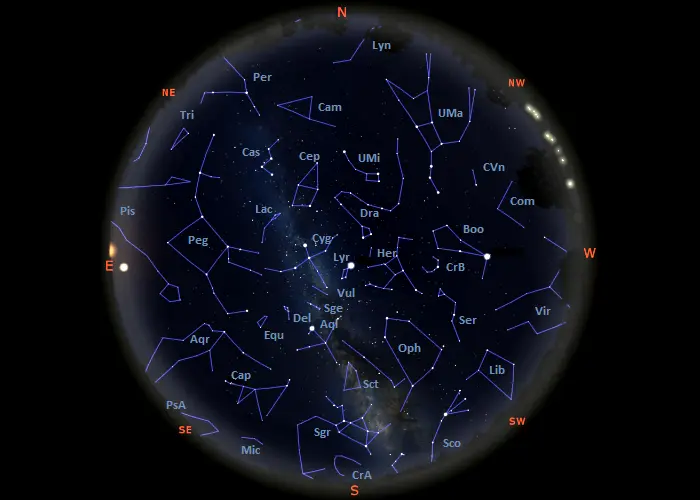
\includegraphics[scale=0.6]{constellations/08.webp.png}
\end{figure}


\newpage
$\;$
\newpage
    \noindent{\Large\sffamily\bfseries Aug, \textbf{\sffamily{24}} Aug - \textbf{\sffamily{30}} Aug}\par
    \enlargethispage{1.2cm}
    \vspace{0.8ex}
    \markboth{Aug, \textbf{\sffamily{24}} Aug - \textbf{\sffamily{30}} Aug}{}
    \setlength{\tabcolsep}{3pt}
    \renewcommand{\arraystretch}{1}
    \noindent\begin{tabularx}{\linewidth}{@{}X X X@{}}
      \calendarDayBlock{Lunes}{\textbf{\sffamily{24}} Aug}{\small{}}{\small{}}{
\includegraphics[width=0.32cm]{moon_phases/Moon_phase_3.svg.png}} &
      \calendarDayBlock{Martes}{\textbf{\sffamily{25}} Aug}{\small{}}{\small{}}{
\includegraphics[width=0.32cm]{moon_phases/Moon_phase_3.svg.png}} &
      \calendarDayBlock{Miércoles}{\textbf{\sffamily{26}} Aug}{\small{}}{\small{}}{
\includegraphics[width=0.32cm]{moon_phases/Moon_phase_4.svg.png}}
    \end{tabularx}

    \vspace{1.75cm}

    \noindent\begin{tabularx}{\linewidth}{@{}X X X@{}}
      \calendarDayBlock{Jueves}{\textbf{\sffamily{27}} Aug}{\small{}}{\small{}}{
\includegraphics[width=0.32cm]{moon_phases/Moon_phase_4.svg.png}} &
      \calendarDayBlock{Viernes}{\textbf{\sffamily{28}} Aug}{\small{}}{\small{}}{
\includegraphics[width=0.32cm]{moon_phases/Moon_phase_4.svg.png}} &
      \calendarWeekendBlock{\textbf{\sffamily{29}} Aug}{\small{}}{\small{}}{
\includegraphics[width=0.32cm]{moon_phases/Moon_phase_4.svg.png}}{\textbf{\sffamily{30}} Aug}{\small{}}{\small{}}{
\includegraphics[width=0.32cm]{moon_phases/Moon_phase_5.svg.png}}
    \end{tabularx}

\newpage    \noindent{\Large\sffamily\bfseries Aug, \textbf{\sffamily{31}} Aug - \textbf{\sffamily{06}} Sep}\par
    \enlargethispage{1.2cm}
    \vspace{0.8ex}
    \markboth{Aug, \textbf{\sffamily{31}} Aug - \textbf{\sffamily{06}} Sep}{}
    \setlength{\tabcolsep}{3pt}
    \renewcommand{\arraystretch}{1}
    \noindent\begin{tabularx}{\linewidth}{@{}X X X@{}}
      \calendarDayBlock{Lunes}{\textbf{\sffamily{31}} Aug}{\small{}}{\small{}}{
\includegraphics[width=0.32cm]{moon_phases/Moon_phase_5.svg.png}} &
      \calendarDayBlock{Martes}{\textbf{\sffamily{01}} Sep}{\small{}}{\small{}}{
\includegraphics[width=0.32cm]{moon_phases/Moon_phase_5.svg.png}} &
      \calendarDayBlock{Miércoles}{\textbf{\sffamily{02}} Sep}{\small{}}{\small{}}{
\includegraphics[width=0.32cm]{moon_phases/Moon_phase_6.svg.png}}
    \end{tabularx}

    \vspace{1.75cm}

    \noindent\begin{tabularx}{\linewidth}{@{}X X X@{}}
      \calendarDayBlock{Jueves}{\textbf{\sffamily{03}} Sep}{\small{}}{\small{}}{
\includegraphics[width=0.32cm]{moon_phases/Moon_phase_6.svg.png}} &
      \calendarDayBlock{Viernes}{\textbf{\sffamily{04}} Sep}{\small{}}{\small{}}{
\includegraphics[width=0.32cm]{moon_phases/Moon_phase_6.svg.png}} &
      \calendarWeekendBlock{\textbf{\sffamily{05}} Sep}{\small{}}{\small{}}{
\includegraphics[width=0.32cm]{moon_phases/Moon_phase_6.svg.png}}{\textbf{\sffamily{06}} Sep}{\small{}}{\small{}}{
\includegraphics[width=0.32cm]{moon_phases/Moon_phase_7.svg.png}}
    \end{tabularx}

\newpage    \noindent{\Large\sffamily\bfseries Sep, \textbf{\sffamily{07}} Sep - \textbf{\sffamily{13}} Sep}\par
    \enlargethispage{1.2cm}
    \vspace{0.8ex}
    \markboth{Sep, \textbf{\sffamily{07}} Sep - \textbf{\sffamily{13}} Sep}{}
    \setlength{\tabcolsep}{3pt}
    \renewcommand{\arraystretch}{1}
    \noindent\begin{tabularx}{\linewidth}{@{}X X X@{}}
      \calendarDayBlock{Lunes}{\textbf{\sffamily{07}} Sep}{\small{}}{\small{}}{
\includegraphics[width=0.32cm]{moon_phases/Moon_phase_7.svg.png}} &
      \calendarDayBlock{Martes}{\textbf{\sffamily{08}} Sep}{\small{}}{\small{}}{
\includegraphics[width=0.32cm]{moon_phases/Moon_phase_7.svg.png}} &
      \calendarDayBlock{Miércoles}{\textbf{\sffamily{09}} Sep}{\small{}}{\small{}}{
\includegraphics[width=0.32cm]{moon_phases/Moon_phase_7.svg.png}}
    \end{tabularx}

    \vspace{1.75cm}

    \noindent\begin{tabularx}{\linewidth}{@{}X X X@{}}
      \calendarDayBlock{Jueves}{\textbf{\sffamily{10}} Sep}{\small{}}{\small{}}{
\includegraphics[width=0.32cm]{moon_phases/Moon_phase_0.svg.png}} &
      \calendarDayBlock{Viernes}{\textbf{\sffamily{11}} Sep}{\small{}}{\small{}}{
\includegraphics[width=0.32cm]{moon_phases/Moon_phase_0.svg.png}} &
      \calendarWeekendBlock{\textbf{\sffamily{12}} Sep}{\small{}}{\small{}}{
\includegraphics[width=0.32cm]{moon_phases/Moon_phase_0.svg.png}}{\textbf{\sffamily{13}} Sep}{\small{}}{\small{}}{
\includegraphics[width=0.32cm]{moon_phases/Moon_phase_1.svg.png}}
    \end{tabularx}

\newpage    \noindent{\Large\sffamily\bfseries Sep, \textbf{\sffamily{14}} Sep - \textbf{\sffamily{20}} Sep}\par
    \enlargethispage{1.2cm}
    \vspace{0.8ex}
    \markboth{Sep, \textbf{\sffamily{14}} Sep - \textbf{\sffamily{20}} Sep}{}
    \setlength{\tabcolsep}{3pt}
    \renewcommand{\arraystretch}{1}
    \noindent\begin{tabularx}{\linewidth}{@{}X X X@{}}
      \calendarDayBlock{Lunes}{\textbf{\sffamily{14}} Sep}{\small{}}{\small{}}{
\includegraphics[width=0.32cm]{moon_phases/Moon_phase_1.svg.png}} &
      \calendarDayBlock{Martes}{\textbf{\sffamily{15}} Sep}{\small{}}{\small{}}{
\includegraphics[width=0.32cm]{moon_phases/Moon_phase_1.svg.png}} &
      \calendarDayBlock{Miércoles}{\textbf{\sffamily{16}} Sep}{\small{}}{\small{}}{
\includegraphics[width=0.32cm]{moon_phases/Moon_phase_1.svg.png}}
    \end{tabularx}

    \vspace{1.75cm}

    \noindent\begin{tabularx}{\linewidth}{@{}X X X@{}}
      \calendarDayBlock{Jueves}{\textbf{\sffamily{17}} Sep}{\small{}}{\small{}}{
\includegraphics[width=0.32cm]{moon_phases/Moon_phase_2.svg.png}} &
      \calendarDayBlock{Viernes}{\textbf{\sffamily{18}} Sep}{\small{}}{\small{}}{
\includegraphics[width=0.32cm]{moon_phases/Moon_phase_2.svg.png}} &
      \calendarWeekendBlock{\textbf{\sffamily{19}} Sep}{\small{}}{\small{}}{
\includegraphics[width=0.32cm]{moon_phases/Moon_phase_2.svg.png}}{\textbf{\sffamily{20}} Sep}{\small{}}{\small{}}{
\includegraphics[width=0.32cm]{moon_phases/Moon_phase_2.svg.png}}
    \end{tabularx}

\newpage\end{document}